\documentclass[a4paper,12pt]{article}
\usepackage{amsmath}
\usepackage{amssymb}
\usepackage[polish]{babel}
\usepackage{polski}
\usepackage[utf8]{inputenc}
\usepackage{indentfirst}
\usepackage{geometry}
\usepackage{array}
\usepackage[pdftex]{color,graphicx}
\usepackage{subfigure}
\usepackage{afterpage}
\usepackage{setspace}
\usepackage{color}
\usepackage{wrapfig}
\usepackage{listings}
\usepackage{datetime}

\renewcommand{\onehalfspacing}{\setstretch{1.6}}

\geometry{tmargin=2.5cm,bmargin=2.5cm,lmargin=2.5cm,rmargin=2.5cm}
\setlength{\parindent}{1cm}
\setlength{\parskip}{0mm}

\newenvironment{lista}{
\begin{itemize}
  \setlength{\itemsep}{1pt}
  \setlength{\parskip}{0pt}
  \setlength{\parsep}{0pt}
}{\end{itemize}}

\newcommand{\linia}{\rule{\linewidth}{0.4mm}}

\definecolor{lbcolor}{rgb}{0.95,0.95,0.95}
\lstset{
  backgroundcolor=\color{lbcolor},
  tabsize=4,
  language=C++,
  captionpos=b,
  tabsize=3,
  frame=lines,
  numbers=left,
  numberstyle=\tiny,
  numbersep=5pt,
  breaklines=true,
  showstringspaces=false,
  basicstyle=\footnotesize,
  identifierstyle=\color{magenta},
  keywordstyle=\color[rgb]{0,0,1},
  commentstyle=\color[rgb]{0,0.5,0},
  stringstyle=\color{red}
}

\begin{document}

\noindent
\begin{tabular}{|c|p{11cm}|c|} \hline
Grupa~4 & Katarzyna Kosiak i~Michał Folwarski & \ddmmyyyydate\today \tabularnewline
\hline
\end{tabular}

\section*{Zadanie~6 -- Liczby pierwsze w~CUDA}
Program ma za zadanie wykonać test pierwszości (sprawdzić czy dana liczba jest liczbą pierwszą) na zestawie liczb zapisanym w~pliku.
Algorytm sprawdzania testu pierwszości został zaimplementowany na bazie metody naiwnej oraz optymalizacji~o:
\begin{lista}
 \item pominięcie liczb parzystych,
 \item pominięcie liczb podzielnych przez trzy,
 \item sprawdzenie dzielników tylko do pierwiastka kwadratowego sprawdzanej liczby.
\end{lista}

\begin{lstlisting}
// alokacja pamieci na karcie graficznej
cudaMalloc((void**) &dev_numbers, numbers.size()*sizeof(struct myNumber));

// kopiowanie danych na karte graficzna
cudaMemcpy( dev_numbers, numbers.data(),
            numbers.size() * sizeof(struct myNumber),
            cudaMemcpyHostToDevice );

// wykonywanie obliczen na karcie graficznej
kernel<<< numbers.size(), 1 >>>( dev_numbers, numbers.size() );

// kopiowanie wynikow z karty gfraficznej
cudaMemcpy( numbers.data(), dev_numbers,
            numbers.size() * sizeof(struct myNumber),
            cudaMemcpyDeviceToHost );
\end{lstlisting}

Powyższy fragment kodu przedstawia główną ideę w~jaki sposób zostało zorganizowane wykonywanie obliczeń na karcie graficznej w~technologii CUDA. W~kernelu jest wykonywany test pierwszości dla każdej liczy, a~ponieważ obliczenia dla każdej liczby można wykonać niezależnie od pozostałych, to najlepszy czas obliczeń uzyskamy gdy będziemy wykonywać test pierwszości dla wszystkich liczb jednocześnie. W~naszym przypadku osiągnęliśmy to poprzez dynamiczne ustawienie ilości bloków dla kernela równej ilości liczb w~danym zestawie liczb do sprawdzenia oraz jeden wątkiem na każdy blok. Wszelkie inne kombinacje z~ilością i~rozmiarami bloków, gdy sumaryczna ilość wątków jest równa wielkości zestawu danych dają takie same rezultaty.

\begin{figure}[!hbp]
\begin{center}
\subfigure[zestaw składający się z~40 liczb]{
    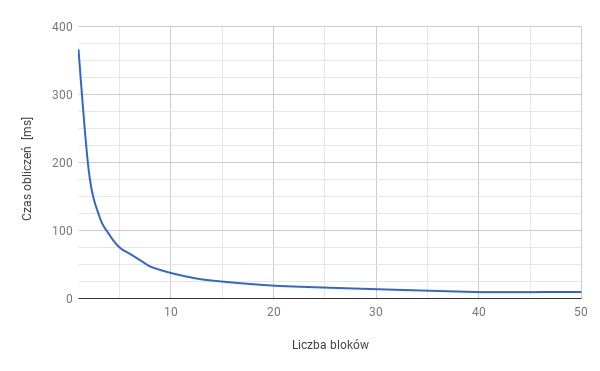
\includegraphics[width=0.45\textwidth]{chart-40}
    \label{chart40}
    }
\subfigure[zestaw składający się z~80 liczb]{
    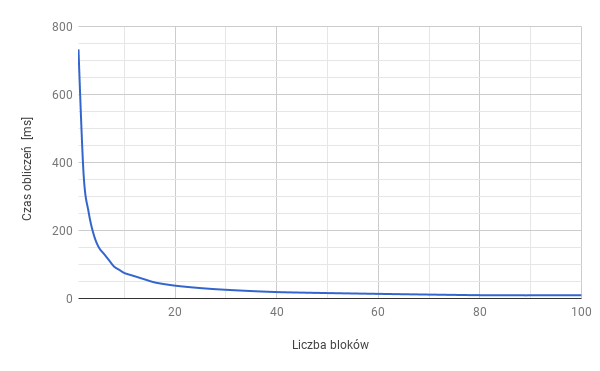
\includegraphics[width=0.45\textwidth]{chart-80}
    \label{chart80}
    }
  \caption{Wykresy zależności czasu wykonania obliczeń od liczby bloków}
\end{center}
\end{figure}
Wykresy na rysunku numer~1 przedstawiają wyniki czasu obliczeń dla dwóch różnych zestawów liczb. Z~wykresów można odczytać, że najlepszy czas osiągamy dla liczby bloków równej wielkości zestawu danych, a~dalsze zwiększanie liczby bloków (ponad rozmiar zestawu danych) nie przynosi wzrostu przyspieszenie -- wyniki nieznacznie się różnią od tego najlepszego.

\begin{figure}[!hbp]
\begin{center}
\subfigure[zestaw składający się z~40 liczb]{
    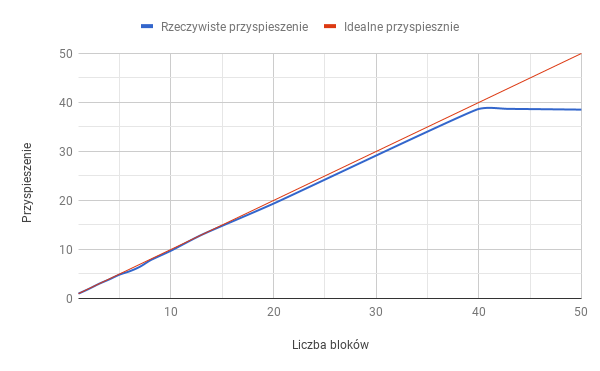
\includegraphics[width=0.45\textwidth]{chart-40-acc}
    \label{chart40-acc}
    }
\subfigure[zestaw składający się z~80 liczb]{
    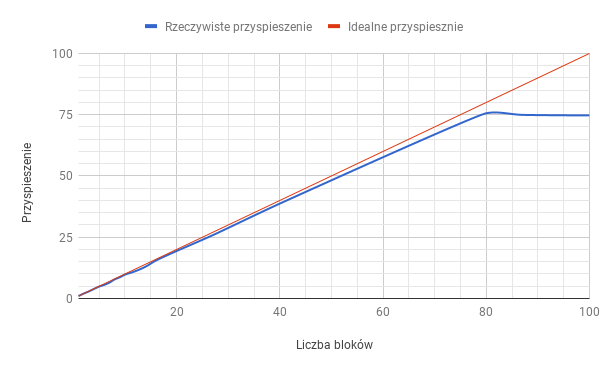
\includegraphics[width=0.45\textwidth]{chart-80-acc}
    \label{chart80-acc}
    }
  \caption{Wykresy przyspieszenia wykonania obliczeń w~zależności od liczby bloków}
\end{center}
\end{figure}
Z powyższych wykresów można odczytać, że maksymalne przyspieszenie dla tych danych wyniosło odpowiednio~38,5 dla zestawu składającego się z~czterdziestu liczb oraz~76,5 dla drugiego zestawu składającego się z~osiemdziesięciu liczb. Czyli w~tych przypadkach uzyskaliśmy przyspieszenie to którego oczekiwaliśmy -- wszystkie liczby były jednocześnie liczone, czyli przyspieszenie wyniosło w~przybliżeniu tyle co ilość liczb w~pliku wejściowym. Uzyskane wyniki przyspieszenia w~dużej mierze zależą od zestawu danych.

\subsubsection*{Wnioski}
\noindent Dzięki wykonywaniu obliczeń na karcie graficznej, możliwe jest znaczne przyspieszenie obliczeń, ponieważ możliwość jednoczesnego uruchomienia obliczeń na karcie graficznej jest znacznie większa niż na procesorze. W~tym zadaniu przetestowaliśmy możliwość dynamicznego rozdzielenia zadań, a~co w~naszym przypadku przyniosło oczekiwane rezultaty -- obliczenia zostały zrównoleglone na karcie graficznej i~dzięki temu zwiększyła się szybkość obliczeń. Dostrzegliśmy też, że ``wąskim gardłem'' w~tej technologii jest przesyłanie danych pomiędzy procesorem a~kartą graficzną -- czas przesyłania danych oscylował w~okolicy 400ms podczas gdy obliczenia na karcie graficznej w~optymalnej konfiguracji wyniosły zaledwie kilka milisekund.

\end{document}
